\chapter{Technical Design Development}\label{ch:techdesdev}


\section{Organisational Breakdown Structure}\label{sec:orgbreakdown}
A clear division of roles and responsibilities is of paramount importance for a functional working environment, hence this chapter establishes all organisational and technical roles each member of the team has. This will be illustrated by an organogram in \cref{fig:orgbreakdownstruc}, and the responsibilities of each role are defined in \cref{sec:org-roles}, as this will keep the organogram as organised and concise as possible. Moreover, the initials of each team member can be seen in each role, clarifying and simplifying the organogram.

\begin{figure}[ht]
    \centering
    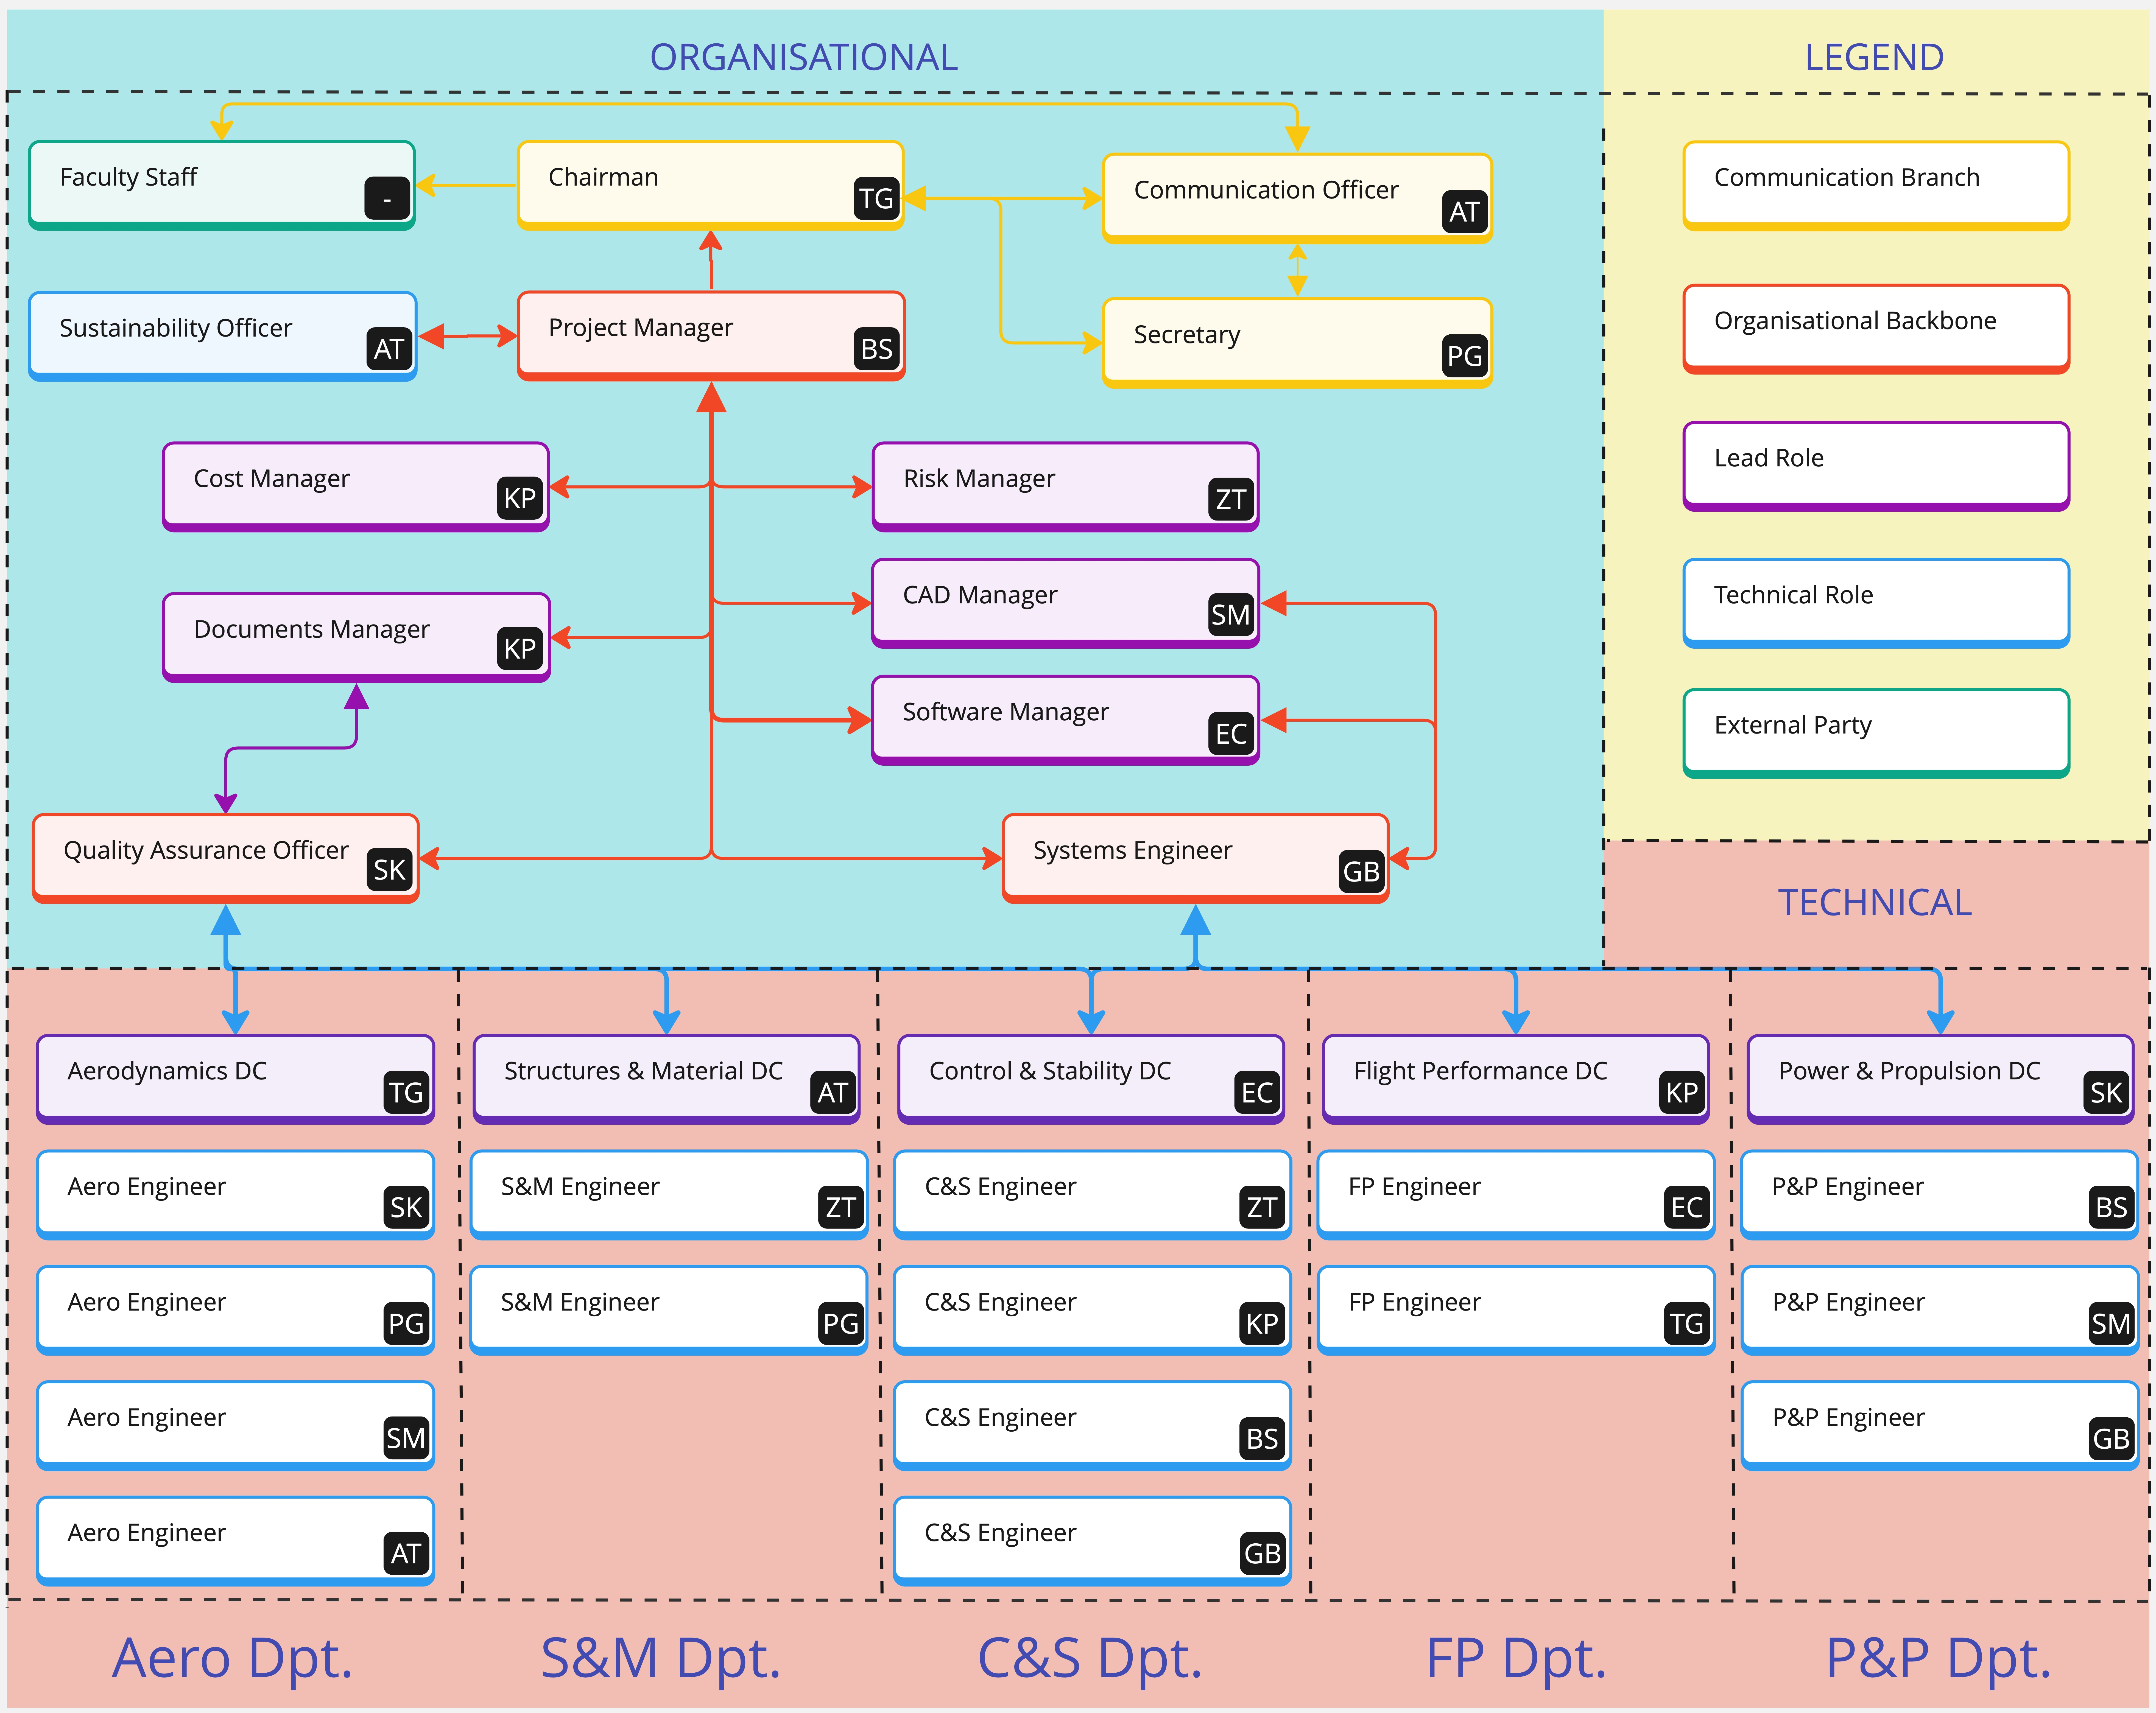
\includegraphics[width=\linewidth]{figures/Copy OBS.jpg}
    \caption{Organisational Breakdown Structure, the abbreviations of the members of the team are specified in .}
    \label{fig:orgbreakdownstruc}
\end{figure}


\subsection{Organisational Roles}\label{sec:org-roles}
The assigned responsibilities for all the organisational roles presented in \cref{fig:orgbreakdownstruc} are specified and elaborated on below:
\begin{itemize}
    \item \textbf{Project Manager (PM)}: The PM coordinates the team, manages resources, and ensures the project meets deadlines, and budgets and regulates proper sharing of information with the outside~\cite{dsePMSESlides1}.
    The responsibilities of the PM can be broken down into:
    \begin{itemize}
        \item \textit{The PM shall define the organisation and procedures of the project, along with ensuring sensible results, budget and resource allocation.}
        \item \textit{The PM shall closely follow and supervise the development of the Gantt Chart and the project schedule.}
        \item \textit{The PM shall constantly collect information on project status to be shared with the interested parties, define and take corrective/adaptive actions, and officially close out the project.}
    \end{itemize}
    \item \textbf{Chairman}: The Chairman, is the main communication link with the external parties, as can be deduced from \cref{fig:orgbreakdownstruc}.
    Furthermore, it oversees and controls the communication branch in its entirety, ensuring clear and effective communication between all the team members.
    The responsibilities of the Chairman can be broken down into:
    \begin{itemize}
        \item \textit{The Chairman shall lead the customer and staff meetings, by directing the discussion according to the meeting.}
        \item \textit{The Chairman shall be responsible for smooth communication with the secretary and communication officer.}
    \end{itemize}
    \item \textbf{Secretary}: The Secretary shall maintain and organise the various tasks, implement procedures and carry out administrative duties~\cite{SysEngrespons}.
    The responsibilities of the Secretary can be broken down into:
    \begin{itemize}
        \item \textit{The Secretary shall always be actively taking notes during meetings and global discussions within the group.}
        \item \textit{The Secretary is responsible for retrieving and preparing the agenda used as a reference for the meetings.}
    \end{itemize}
    \item \textbf{Communication Officer (CO)}: The CO is, besides the Chairman, the sole other member who is in direct communication with the faculty staff and other external parties, mainly through online communication (e.g. via e-mail).
    The responsibilities of the CO can be broken down into:
    \begin{itemize}
        \item \textit{The CO provides direct communication between the faculty staff and team, hence he is also responsible for a clear meeting schedule.}
        \item \textit{The CO shall ensure constant effective communication between all the team members.}
    \end{itemize}
    \item \textbf{Sustainability Officer (SO)}: The SO is responsible for guiding the team's effort towards an environmental, social and economical-conscious working approach~\cite{sustofficer}.
    As this is one of the greater areas of focus of the team, during the project;
    \item \textbf{Quality Assurance Officer (QAO)}: The QAO, alongside the SE, provides a clear connection between the organisational and technical sections of the organogram.
    Hence, the QAO has to be in clear and direct communication with the SE to ensure quality in the technical division.
    The responsibilities of the QAO can be broken down into:
    \begin{itemize}
        \item \textit{The QAO shall perform frequent, standardised and planned quality controls concerning content and progress of the project.}
        \item \textit{The QAO shall provide clear guidelines for writing and organisational and technical procedures.}
        \item \textit{The QAO shall provide the team with a clear plan to make the proofreading process as thorough and efficient as possible.}
    \end{itemize}
    \item \textbf{Systems Engineer (SE)}: The SE is responsible for the correct integration of complex systems, ensuring all components work together effectively to meet project requirements and objectives~\cite{SysEngrespons}.
    The responsibilities of the SE can be broken down into:
    \begin{itemize}
        \item \textit{The SE shall evaluate the current systems and identify and implement potential improvements.}
        \item \textit{The SE is in charge of the installation, configuration, improvement and monitoring of new systems, and monitors the implications that the systems usage has on the project.}
%        \item \textit{Coordination of affected departments and other interested parties, including the potential need for training.}  % should be removed I think, training is pretty for fetched for such a short project
%        \item \textit{Collaboration with team members, end users, clients, suppliers, and stakeholders with a focus on continuous improvement.}
        \item \textit{The SE shall integrate new systems within existing infrastructures, emphasising advantages, and minimising disruption.}
        \item \textit{The SE shall communicate the performance levels to management, often via presentations.}
    \end{itemize}
    \item \textbf{Documents Manager (DM)}: The DM shall make sure all the documents used within the project meet standards of quality, objectiveness, and accuracy, and that the industry and the scientific community officially recognise them.
    The responsibilities of the DM can be broken down into:
    \begin{itemize}
        \item \textit{The DM shall ensure that all the documents are of high scientific quality.}
        \item \textit{The DM shall also hold and maintain an archive with all the used documents, ensuring the team's process can be easily validated and traced back to official literature and references.}
        \item \textit{The DM shall also be responsible for the quality of the references used in the report.}
    \end{itemize}
    \item \textbf{Cost Manager (CM)}: The CM is responsible for monitoring and controlling project costs, developing and maintaining budget forecasts, identifying cost-saving opportunities, and ensuring the project remains within financial constraints while meeting its objectives and quality standards;
    \item \textbf{Risk Manager (RM)}: The RM is responsible for the identification, assessment, analysis, and handling of all possible risks, ensuring proper risk management over the entire team.
    \begin{itemize}
        \item \textit{The RM shall provide a methodology to identify, assess, analyse and handle (track, reduce or eliminate) all the possible risks.}
        \item \textit{The RM shall apply this methodology within each department to ensure proper risk management over the entire team.}
        \item \textit{The RM shall draft and further analyse the risk report.}
    \end{itemize}
    \item \textbf{Computer-Aided Design Manager (CADM)}: The CADM shall oversee the use of CAD software, and ensure that all drawings conform to the same standards and regulations.
    \begin{itemize}
        \item \textit{The CADM shall manage the CAD technicians, and ensure the accuracy and quality of all design drawings, as well as ensuring conformity to industry standards and regulations.}
        \item \textit{The CADM shall develop and implement CAD standards and workflows to optimize design processes and facilitate efficient project execution.}
        \item \textit{The CADM shall oversee the use of CAD software and hardware, and ensure that the CAD technicians are properly trained and equipped to use the software and hardware.}
    \end{itemize}
    \item \textbf{Software Manager (SM)}: the SM oversees the development, implementation, and maintenance of software systems
    \begin{itemize}
        \item \textit{The SM shall oversee the software systems' development, implementation, and maintenance.}
        \item \textit{The SM shall manage and fit the department-specific software writing within project timelines, and resources, whilst collaborating with project stakeholders to ensure the software meets all technical specifications and operational requirements.}
        \item \textit{The SM shall ensure that the software is developed according to the project's requirements and specifications.}
        \item \textit{The SM shall ensure that the software engineers are properly trained, and adhere to the project's software development standards, procedures and regulations.}
    \end{itemize}
\end{itemize}


\subsection{Technical Roles}\label{sec:technical-roles}
Before assigning the responsibilities of the technical roles shown in \cref{fig:orgbreakdownstruc}, it is important to specify the departments, which each have their own department chief (DC) directing their specialised engineers.
The team decided to divide the technical tasks into five departments: \textbf{Aerodynamics}, \textbf{Structures \& Materials}, \textbf{Control \& Stability}, \textbf{Flight Performance}, and \textbf{Power \& Propulsion}.
These are considered to be the main areas of focus during the project. 
The DCs are responsible for the coordination of their respective department, as can be deduced from \cref{fig:orgbreakdownstruc}.
Although focused towards coordination and management, the roles of the DCs will not clash with the SE, as the latter will mainly act as coordinator of all the DCs; ensuring correct implementation of the concept of Concurrent Engineering.
Moreover, the specified technical roles have not yet been established, as this will become more clear during the project.
However, the team did divide departments among the interests and expertise, to realise an efficient and healthy working environment.


\section{Project Logic Diagrams}\label{sec:projlogicdiag}
This section dives into the Logic Diagrams used to organise and control the project.
Tools like, the Work Flow Diagrams (WFD), Work Breakdown Structures (WBS), and Gantt Charts are crucial for completing a multi-disciplinary product development project successfully.
The Work Flow Diagram is presented and explained in \cref{sec:wfd}, the Work Breakdown Structure in \cref{sec:wbs}, and the Gantt Chart in \cref{sec:gantt-chart}.

\subsection{Work Flow Diagram}\label{sec:wfd}
To create a proper plan for the time frame and logic of the project, a Work Flow Diagram (WFD) is created.
It illustrates all the relevant deliverables of the project, as well as the necessary activities that are to be performed throughout the project.
A crucial aspect showcased with the help of the WFD is the relationship between different modules (activities or deliverables) of the project.
Thus, iterative activities can be showcased and predicted when organising the project.
Additionally, the WFD displays the responsible person for checking the progress of each of the main tasks.
Moreover, the total work effort required for each of the tasks, as well as the throughput time, are presented in the diagram.

To showcase the flow of the project more clearly, the project is split into six phases, and the flow between the phases and the main deliverables shall be presented in a reduced WFD present at the top of both pages, meant to showcase the project flow.
Afterwards, each of the six phases shall be presented in more detail by showcasing the inputs and outputs, and the constituent elements of every phase, as well as their interrelations.
All elements in the WFD are colour-coded, and referenced in the legend on both pages.

\afterpage{
    \KOMAoptions{paper=A3,paper=portrait,pagesize}
    \recalctypearea
    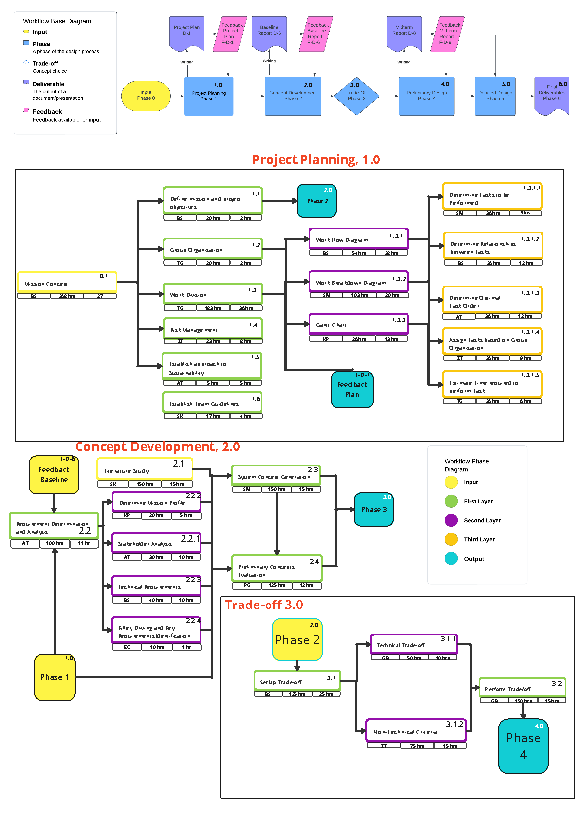
\includepdf{figures/workflowP1.pdf}
    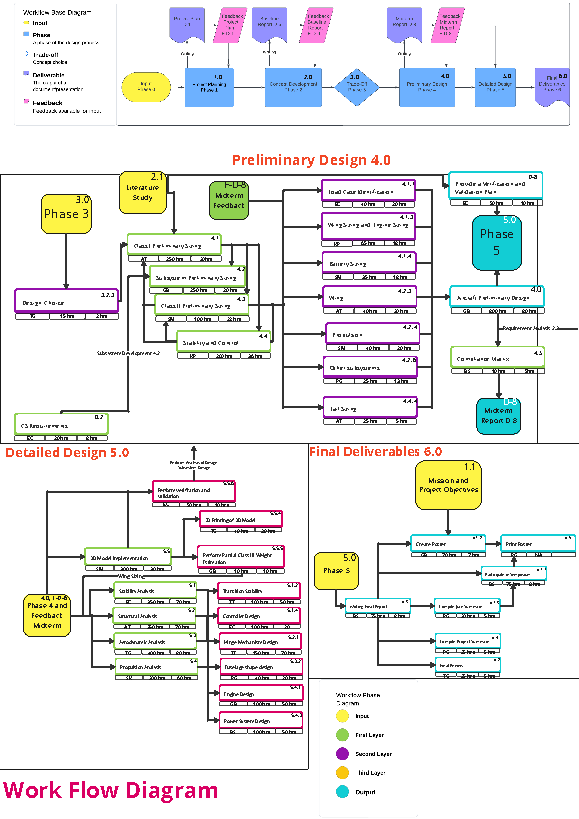
\includepdf{figures/workflowP2.pdf}
    %\clearpage
    \KOMAoptions{paper=A4,paper=portrait,pagesize}
    \recalctypearea
}

\subsection{Work Breakdown Structure}\label{sec:wbs}
From the WFD described in \cref{sec:wfd}, it is possible to derive the Work Breakdown Structure (WBS). This is an invaluable tool in project management, showcasing every phase and task that needs to be completed.
This diagram inherits the top layers of the project phases from the WFD and then breaks these layers into smaller tasks that can be visualized hierarchically. 
Like in the WFD, the responsible person, total time, and throughput time are displayed for every task in the WBS.
% Thanks to the WBS not only all the major processes of the project can be visualized, but it can also be used to create a Gantt chart, as will be explained later.

It is important to note that the sum of the hours in the Work Breakdown Structure does not equal 4000. This is because 300 man-hours are reserved for the PMSE lectures, the peer review of other reports, and the baseline and mid-term review meetings.
\afterpage{
    \KOMAoptions{paper=A3,paper=portrait,pagesize}
    \recalctypearea
    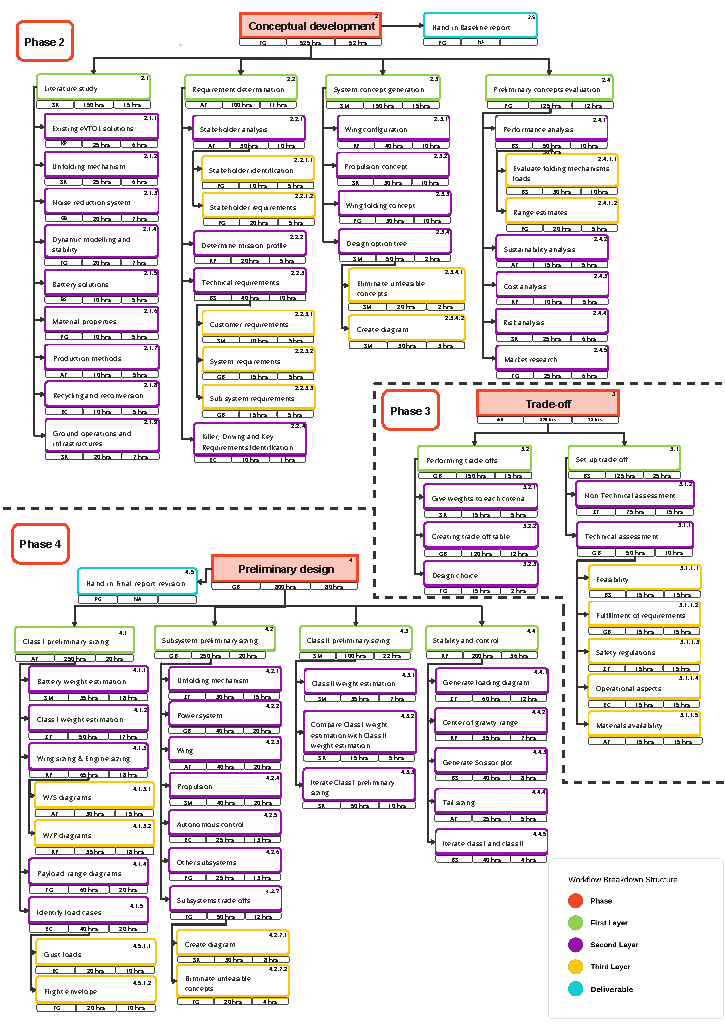
\includepdf{figures/breakdownP1.pdf}
    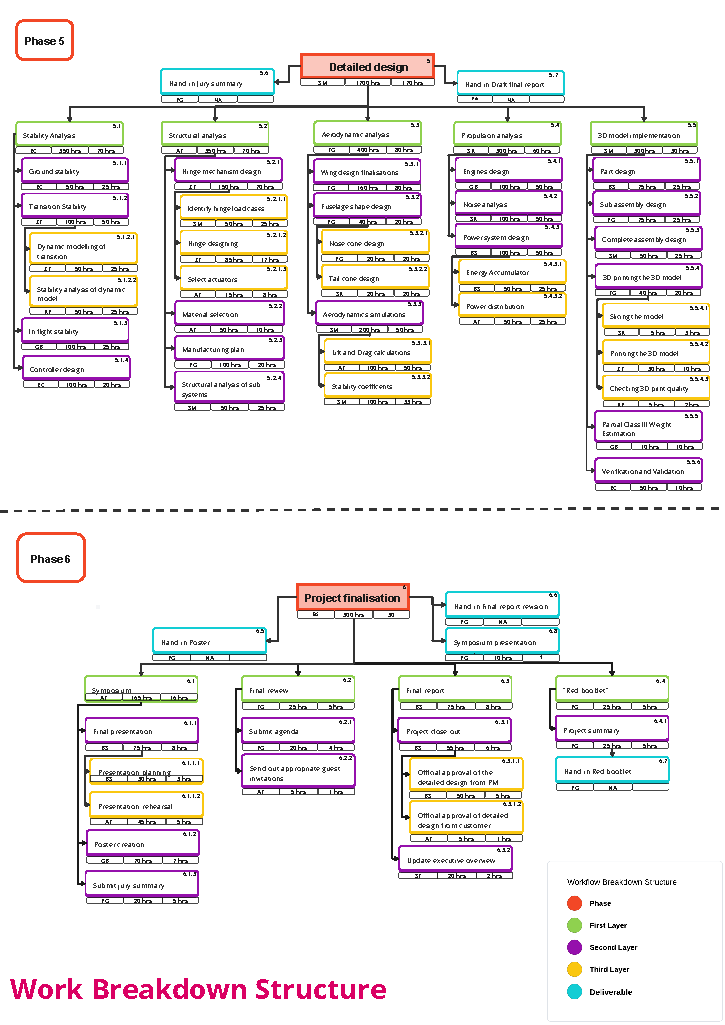
\includepdf{figures/breakdownP22.pdf}
    \KOMAoptions{paper=A4,paper=portrait,pagesize}
    \recalctypearea
}

\subsection{Gantt Chart}\label{sec:gantt-chart}
For the project planning a Gantt Chart was made. The Gantt Chart contains almost 200 tasks. Planning everything to the smallest detail is deemed unnecessary and counterproductive at this point in the design process. That is why only for the next project phase, the concept development phase, all tasks are planned in detail. For the subsequent phases of the project, the main structure is laid out. 

\afterpage{
    \KOMAoptions{paper=A3,paper=landscape,pagesize}
    \recalctypearea
    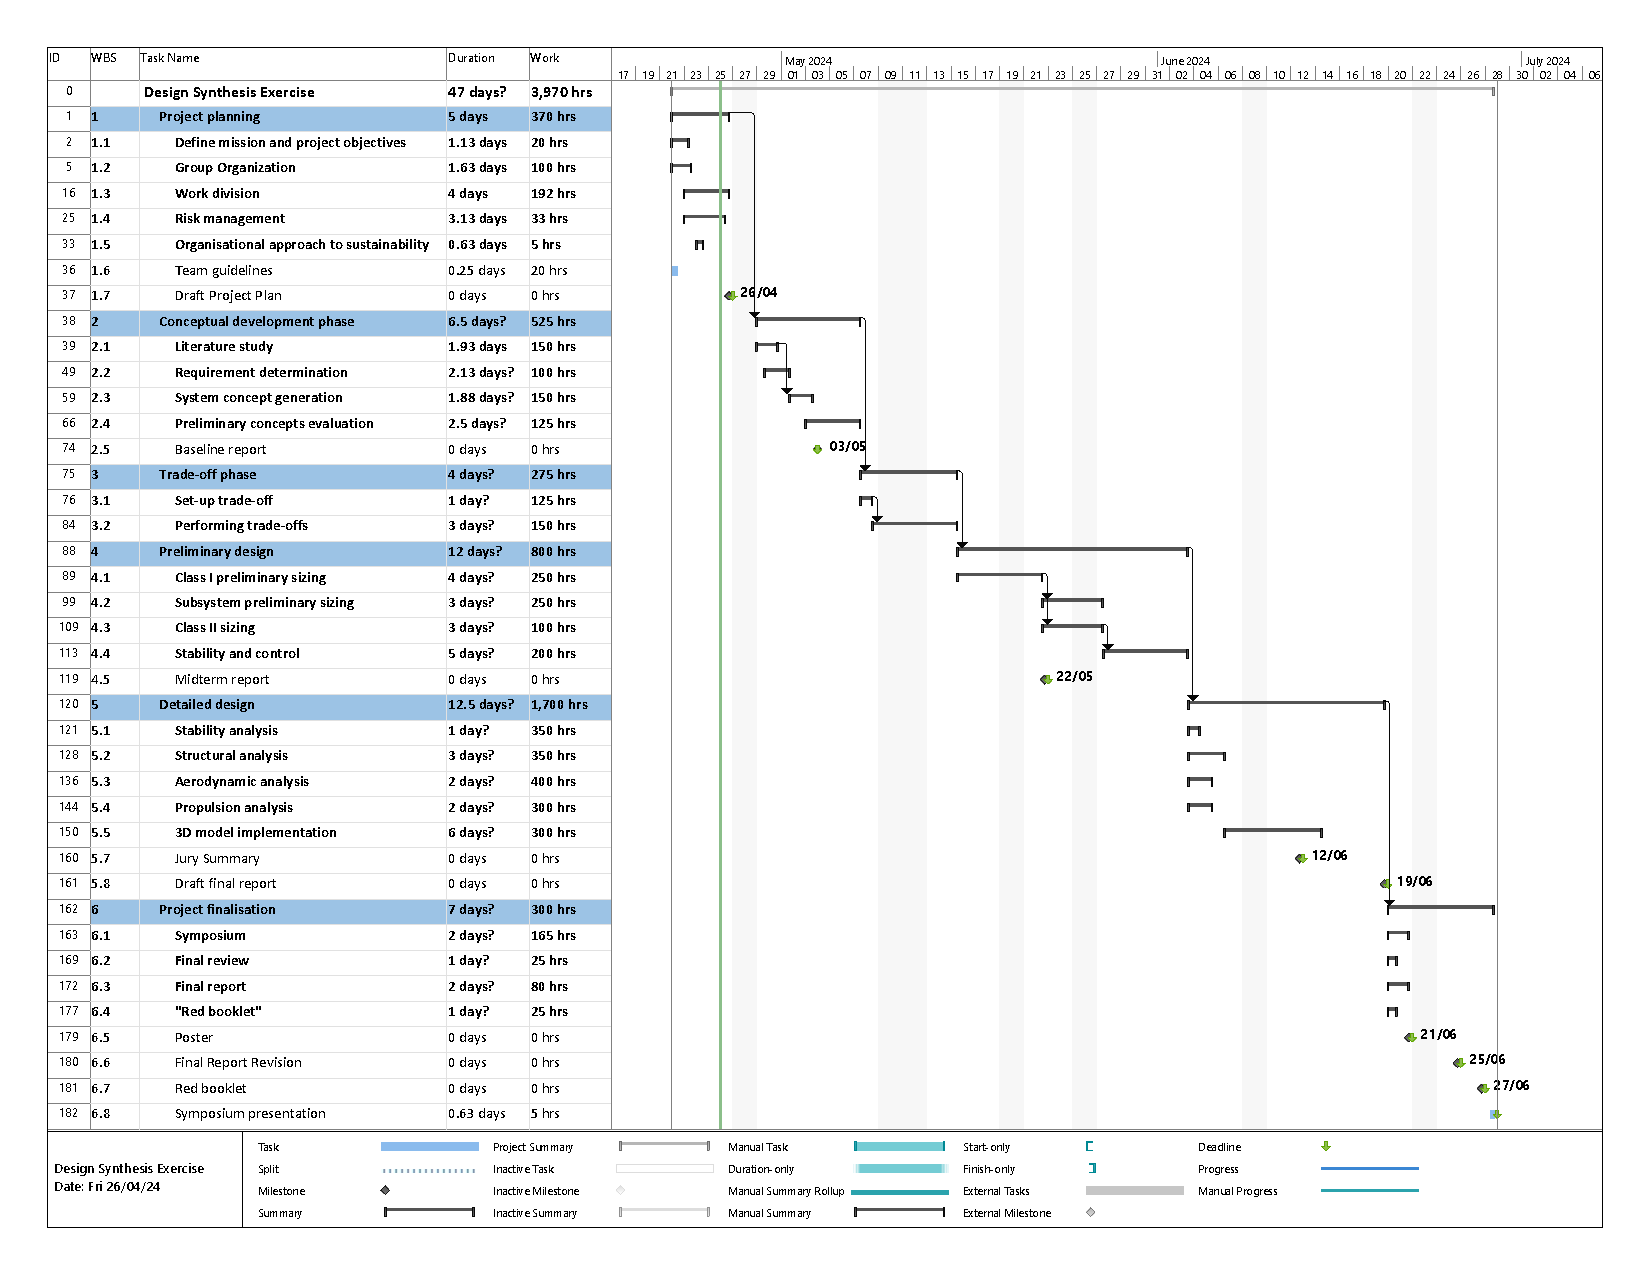
\includepdf{figures/AE3200-Gantt-chart-overall-26042024.pdf}
    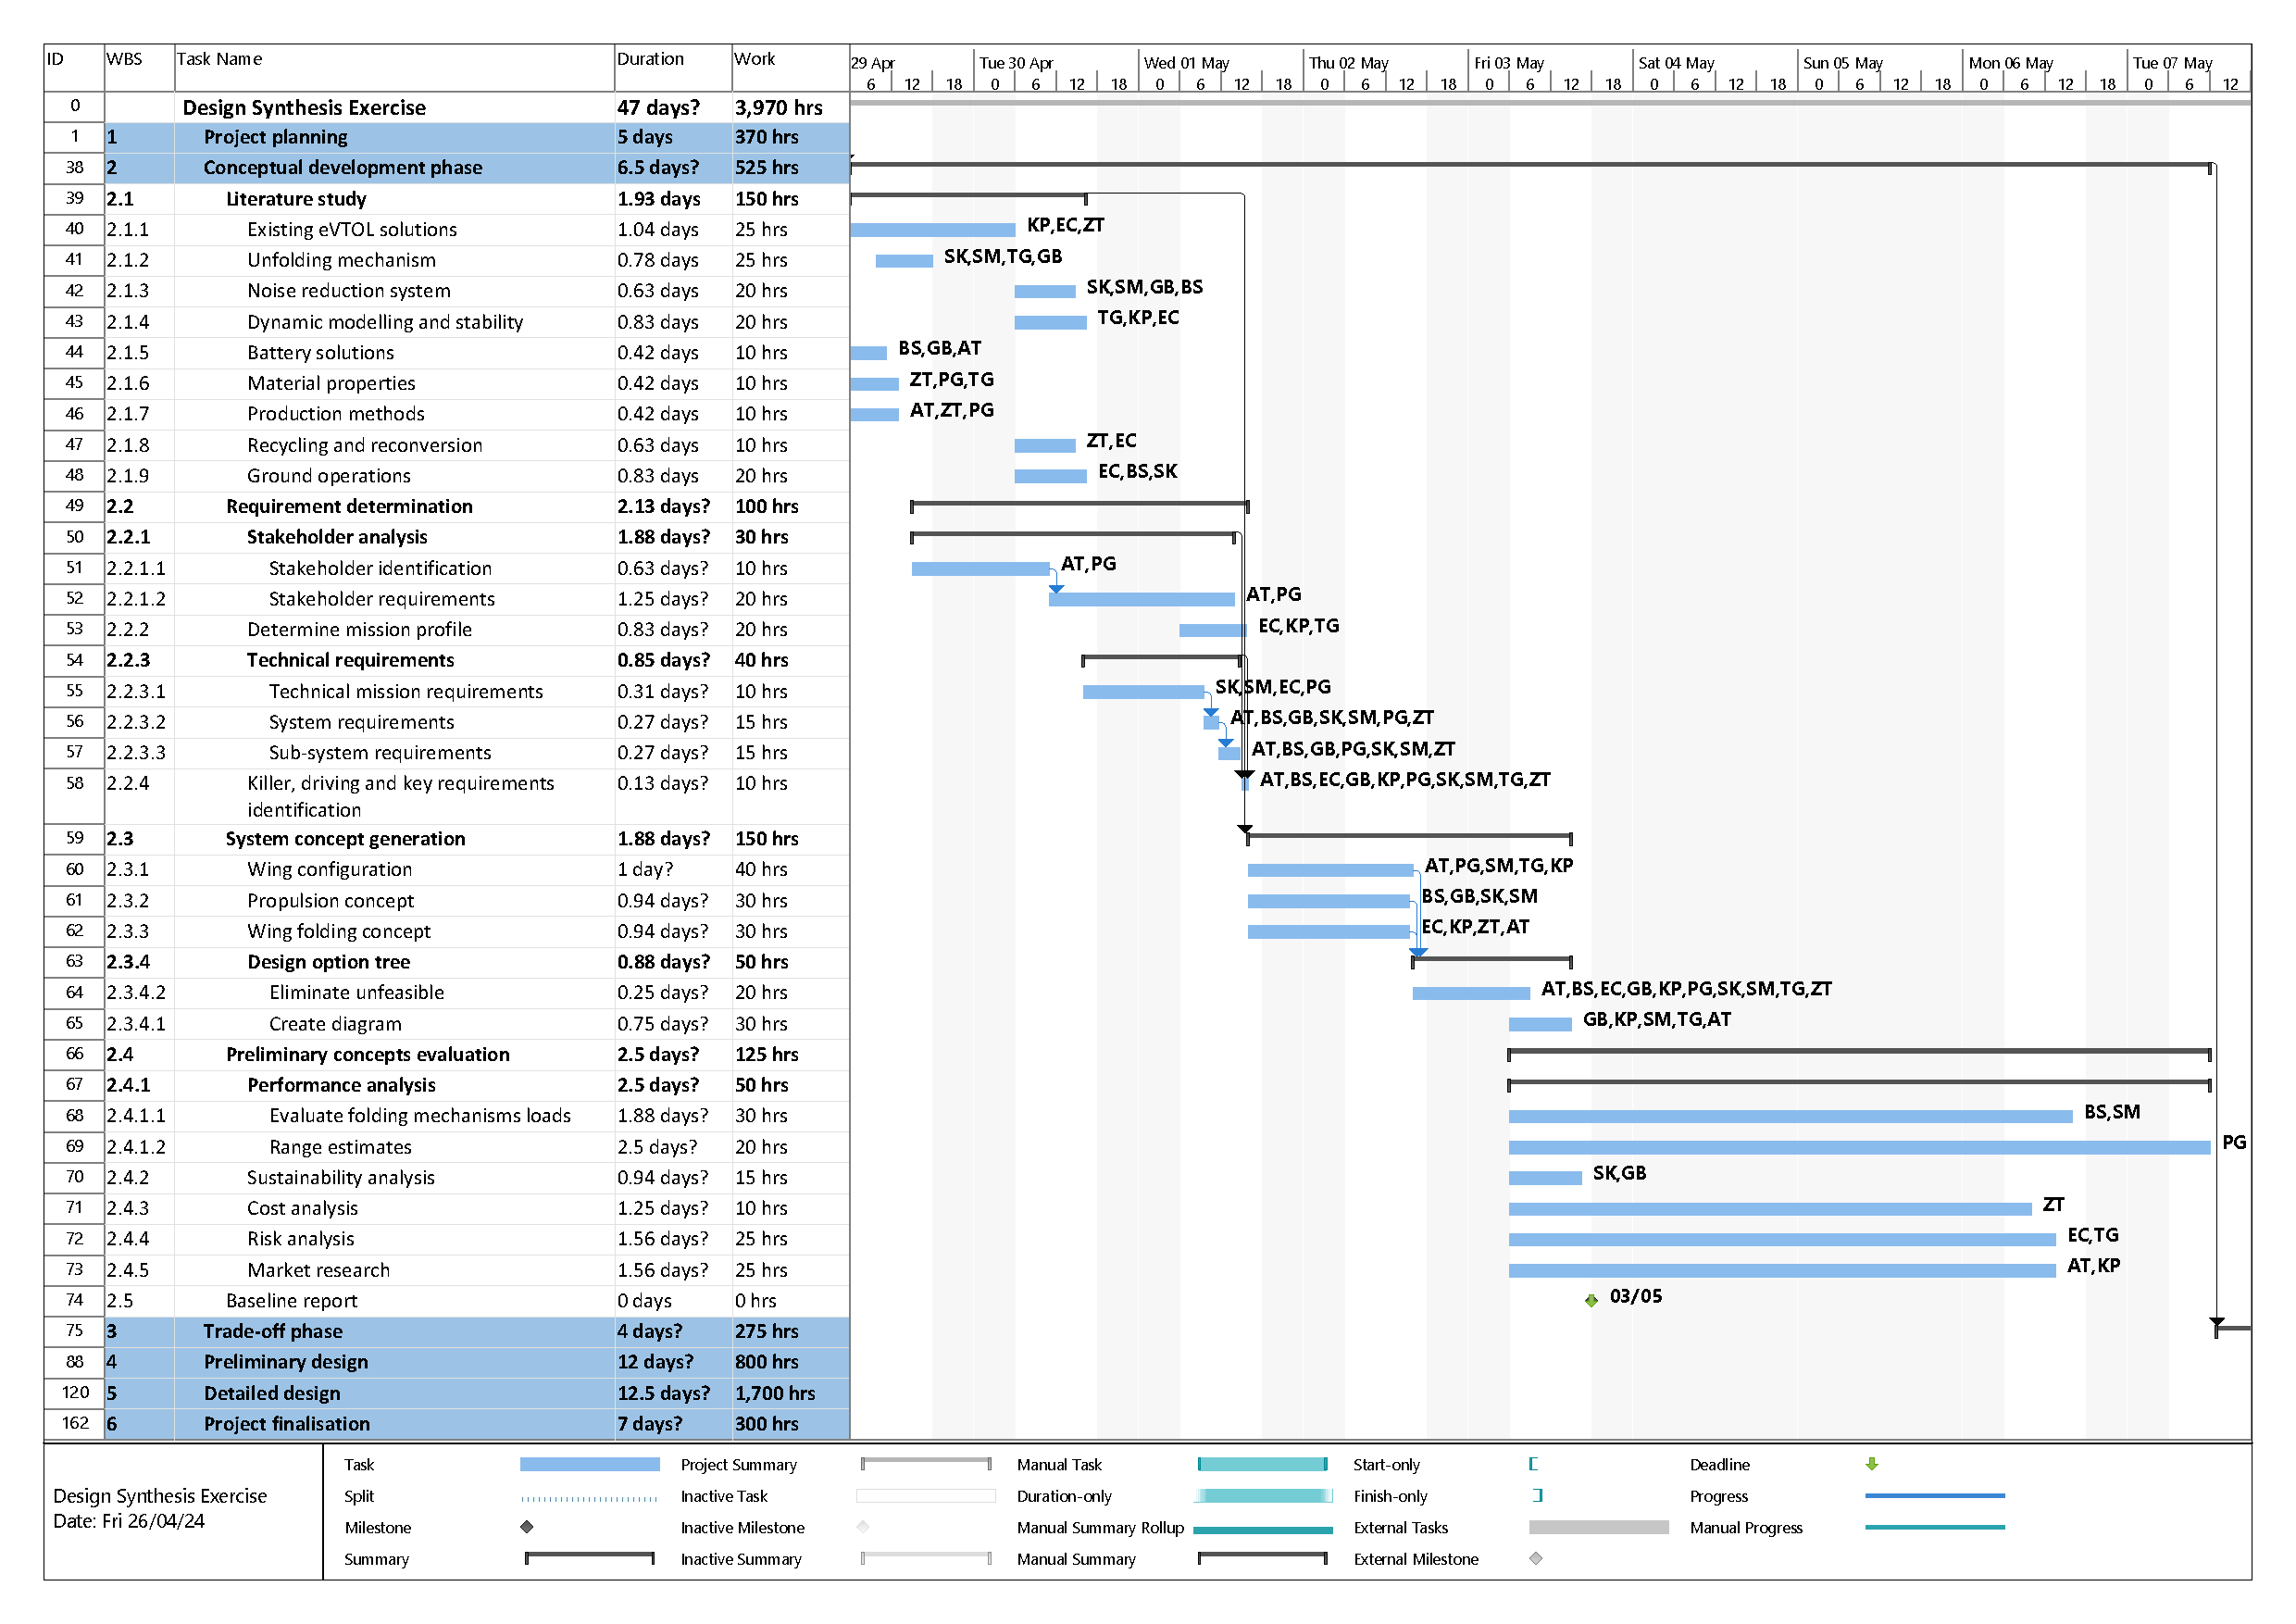
\includepdf{figures/AE3200-Gantt-chart-phase2-26042024.pdf}
    \KOMAoptions{paper=A4,paper=portrait,pagesize}
    \recalctypearea
}
\recalctypearea
